\documentclass[12pt]{article}%
\usepackage{amsfonts}
\usepackage{fancyhdr}
\usepackage{xcolor}
\usepackage[a4paper, top=2.5cm, bottom=2.5cm, left=2.2cm, right=2.2cm]%
{geometry}
\usepackage{amsmath}
\usepackage{changepage}
\usepackage{enumitem}
\usepackage{amssymb}
\usepackage{graphicx}
\usepackage{inconsolata}
\usepackage{hyperref}
\hypersetup{
    colorlinks=true,
    linkcolor=blue,
    filecolor=magenta,      
    urlcolor=blue,
}
\usepackage{listings}
\setcounter{MaxMatrixCols}{30}
\newtheorem{theorem}{Theorem}
\newtheorem{acknowledgement}[theorem]{Acknowledgement}
\newtheorem{algorithm}[theorem]{Algorithm}
\newtheorem{axiom}{Axiom}
\newtheorem{case}[theorem]{Case}
\newtheorem{claim}[theorem]{Claim}
\newtheorem{conclusion}[theorem]{Conclusion}
\newtheorem{condition}[theorem]{Condition}
\newtheorem{conjecture}[theorem]{Conjecture}
\newtheorem{corollary}[theorem]{Corollary}
\newtheorem{criterion}[theorem]{Criterion}
\newtheorem{definition}[theorem]{Definition}
\newtheorem{example}[theorem]{Example}
\newtheorem{exercise}[theorem]{Exercise}
\usepackage{hyperref}

\usepackage{minted}
\newtheorem{lemma}[theorem]{Lemma}
\newtheorem{notation}[theorem]{Notation}
\newtheorem{problem}[theorem]{Problem}
\newtheorem{proposition}[theorem]{Proposition}
\newtheorem{remark}[theorem]{Remark}
\newtheorem{solution}[theorem]{Solution}
\newtheorem{summary}[theorem]{Summary}
\newenvironment{proof}[1][Proof]{\textbf{#1.} }{\ \rule{0.5em}{0.5em}}

\newcommand{\Q}{\mathbb{Q}}
\newcommand{\R}{\mathbb{R}}
\newcommand{\C}{\mathbb{C}}
\newcommand{\Z}{\mathbb{Z}}

\begin{document}

\title{Homework Assignment 5}
\author{CSE 251A: Introduction to Machine Learning}
\date{}
\maketitle

%%%% Deadline
\noindent \textbf {Due: June 8nd, 2022, 9:30am (Pacific Time)} \\


%%%% Instructions.
\noindent \textbf {Instructions:} Please answer the questions below, attach your code in the document, and insert figures to create \textbf{a single PDF file}. \\

\noindent Grade: \underline{\hspace{.8cm}} out of 120 points 








\section{Activation functions (40 Points)}
\begin{enumerate}
    \item Which one of these is a valid layer? For this question, \verb+w.shape=(input, output)+ with \verb+x.shape=(batch size, input)+ and \verb+b.shape=(1, output)+. Note, below that anywhere we use dot, we could have instead used matmul.
        \begin{enumerate}[label=(\alph*)]
            \item \texttt{z = activationFunction(np.dot(x, b) + w)}
            \item \texttt{z = activationFunction(np.dot(x, w)) + b}
            \item \texttt{z = activationFunction(np.dot(x, w) + b)}
        \end{enumerate}
    \item Name at least two possible activation functions and explain the reason why they are used as activation functions.
    \item What will happen if the activation function is a linear function in Multi-layer Perceptron?
\end{enumerate}






\newpage
\section{Overfitting and Regularization (30 Points)}
\begin{enumerate}
    \item What are the common techniques to alleviate overfitting in the neural network training? 
    \item Can we still apply the L1/L2 regularization in NN? If we can, how; if we cannot, why?
\end{enumerate}






\newpage
\section{Compute output for a Convolutional Neural Network (30 Points)}
Consider the image X and filter F given below. Let X be convolved with F
using no padding and a stride of 1 to produce an output Y . What is the
output Y ?

\begin{equation*}
    X = \begin{bmatrix}
        1 & 0 & -2 & 3 & 4 & 1\\
        2 & 9 & 5 & 6 & 0 & -1\\
        0 & -3 & 1 & 3 & 4 & 4\\
        6 & 5 & 2 & 0 & 6 & 8\\
        -5 & 4 & -3 & 1 & 3 & -2\\
        4 & 1 & 2 & 8 & 9 & 7
        \end{bmatrix}
\end{equation*}

\begin{equation*}
    F = \begin{bmatrix}
        -1 & -1 & -1\\
        -1 & 8 & -1 \\
        -1 & -1 & -1
        \end{bmatrix}
\end{equation*}




\newpage
\section{(\textbf{Bonus}, 20 points) Experiment with CNN using Keras}

In this question, you will experiment with Convolutional Neural Networks using the deep learning framework Keras (\url{https://keras.io/api/} ). Please download the Jupyter notebook \texttt{HW5\_CNN.ipynb} and fill in the blanks and answer the questions.  Please attach your \textbf{code} and \textbf{answers} in Gradescope submission.

\textbf{Note: } Make sure this notebook is launched in an environment with Numpy, Tensorflow, matplotlib and Keras installed. You can refer to: \url{https://www.tutorialspoint.com/keras/keras_installation.htm} if you need help with creating a virtual environment with all required dependencies.


\newpage
\section{(20 points) Convolution with padding and dilation.}
In Lecture 15, slide 12 (and Q3 of this assignment) we have gone through the process of calculating the output size of a convolutional layer. Besides the height and width, dilation, stride, and padding are also important parameters of a CNN layer. 
\begin{itemize}
    \item dilation controls the spacing between the kernel points; also known as the atrous algorithm.
    \item stride controls the stride for the cross-correlation, a single number or a tuple.
    \item padding controls the amount of padding applied to the input's outer edges.
\end{itemize}
This \hyperlink{https://github.com/vdumoulin/conv_arithmetic/blob/master/README.md}{link} provides a great visualization of what each parameter controls.


\begin{enumerate}
    \item Given an input of size (16, 16), a filter of size (2, 2) with \texttt{stride=2, padding=1, dilation=4}, what's the output size of it after a \textbf{one} layer 2d-convolution?
    \item Given an input of size (32, 32), a filter of size (3, 3) with \texttt{stride=2, padding=1, dilation=1}, what's the output size of it after a \textbf{two} layer 2d-convolution?
    \item (\textbf{Receptive Field}) The Receptive Field (RF) is defined as the size of the region in the input or previous layers that produce the current feature. For example, Figure \ref{fig:my_label} shows a 3-layer network of filter size (3, 3), with \texttt{stride=1, padding=2, dilation=1}. The receptive field in layer 2 for position (2, 2) of layer 3 is  $3 \times 3=9$, namely, position (1, 1), (1, 2), (1, 3), (2, 1), (2, 2), (2, 3), (3, 1), (3, 2), (3, 3) of layer 2.
    
    When we want to figure out the RF in layer 1, we need to take the \textbf{union} of the receptive field, i.e. the 9 positions, in layer 2. \textbf{Question}: assumed the input is large enough, say, (1000, 1000), what's the size of the receptive field in layer 1 for the position (2, 2) of layer 3? 
\end{enumerate}

\begin{figure}[h]
    \centering
    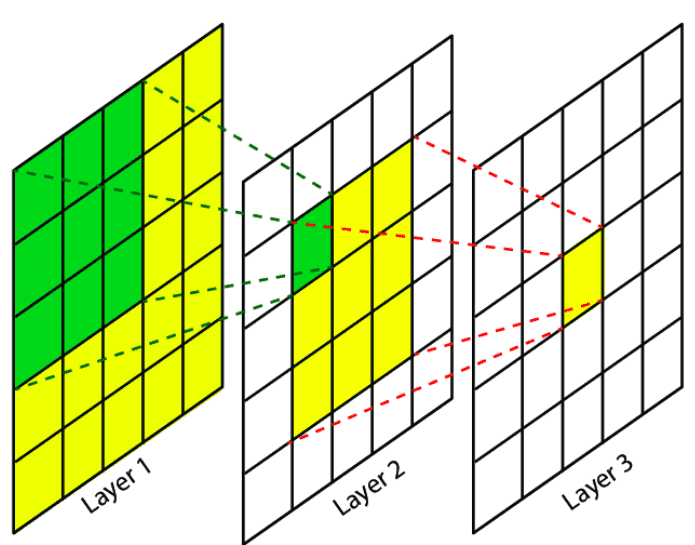
\includegraphics[width=0.3\linewidth]{HW5/receptive-field-in-convolutional-networks.png}
    \caption{Example of RF for a 3-layer CNNs.}
    \label{fig:my_label}
\end{figure}
%\newpage
%\section{(20 points) Convolution? Correlation?}

%In Convolutional Neural Networks, we use convolutional layers to convolute the inputs with the filters. However, in mathematics, there are several ways to combine two (discrete/continuous) functions together. Namely, functional convolution and cross-correlation (details \& definitions can be found \hyperlink{https://en.wikipedia.org/wiki/Convolution}{here}). 

%Determine which operation was used in CNN, and explain why that operation was used instead of the other one.







\end{document}